\section{Lifetime measurements and Coulomb Excitation}

\textbf{a)} To extract the lifetime of the decay from the data given on the question paper, it is necessary to plot the given normalised gamma intensity in terms of its time of flight, shown in \autoref{fig:expo} as red circles. 

Since the recoil is moving at $v = 0.043\unit{c}$, relativistic effects can be ignored. It is possible to convert the given distances flown to times of flight by simply using $t = x/v$. With that, an intensity-time of flight plot can be drawn and fitted to an exponential decay curve of the type:
\begin{equation}
    \label{eq:exponential}
    f(t) = a\exp{\left(\frac{-t}{\tau}\right)},
\end{equation} where $\tau$ is the mean lifetime and $a$ is a constant that should be 1 when using the normalised intensities.

To account for the possibility of several decays happening for the same recoil, which are statistically more likely to be short-lived in comparison with the main decay transition, the first three points have been given a smaller weight than all other points.

\begin{figure}[ht]
    \centering
    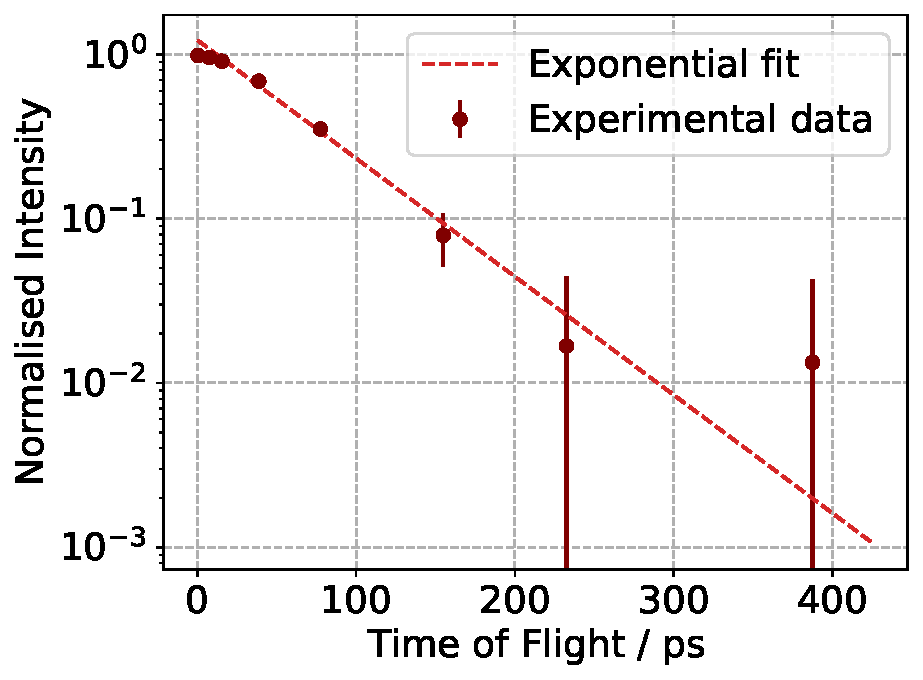
\includegraphics[width=0.9\textwidth]{lifetime.pdf}
    \caption{Normalised intensities as a function of time of flight. The circles are the experimental points given in the question paper and the dotted line is the exponential fit, \autoref{eq:exponential}.}
    \label{fig:expo}
\end{figure}

A different possible approach would have been to fit a convolution of several exponential decays. However, the statistical error introduced with that method would be larger than the one introduced by fitting to a single exponential.

The fitting was performed using \textit{Python}'s package \textit{SciPy} \cite{scipy}. The mean lifetime obtained from the fit is $\tau = 60.3(36)\unit{ps}$. 

\textbf{b)} To use the Differential Decay Curve Method (DDCM) for this data, an approximately straight section of the plot can be chosen to calculate the derivative of the curve as the slope of that straight section. The section limits are shown in \autoref{fig:ddcm} by vertical, dotted lines. The curves were extracted pointwise using \textit{WebPlotDigitizer}~\cite{wpd}.

The average difference between states, $\bar \Delta$, is 0.3, whereas the derivative is calculated pointwise as finely as possible, simply as the difference in intensity between consecutive points divided by the difference in time of consecutive points: $m_i = (y_{i}-y_{i-1})/(x_{i}-x_{i-1})$. The average of the pointwise-calculated slope is taken, $\bar m = \frac{1}{n}\sum_i m_i$. The DDCM mean lifetime is then estimated as:
\begin{equation}
    \label{eq:ddcmlife}
    \tau_{DDCM} = \frac{\bar \Delta}{\bar m} = 56(13)\unit{ps},
\end{equation} where the error is computed roughly as the statistical uncertainty of the averaging process.

\begin{figure}[ht]
    \centering
    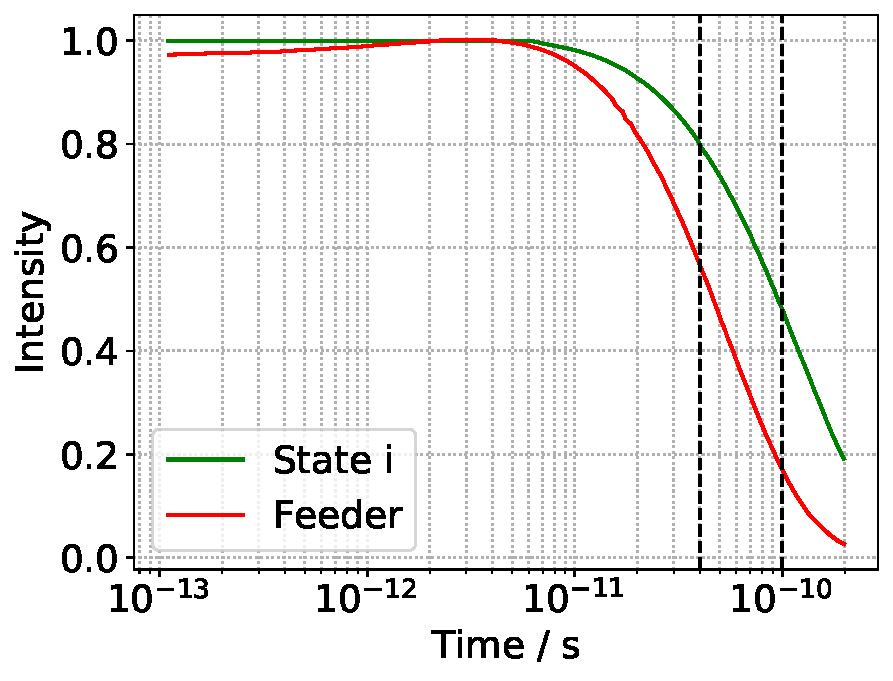
\includegraphics[width=0.75\textwidth]{ddcm.pdf}
    \caption{Curves shown in the question paper, with dotted lines representing the sections used as limits for the section considered for derivation.}
    \label{fig:ddcm}
\end{figure}
\newpage
\textbf{c)} Using the lifetime $\tau = (8.00\pm0.05)\unit{ps}$ and the energy of the first quadrupole state of \ce{^{208}Rn} ($2^+$, 635.8\unit{keV})~\cite{Rn}, it is possible to extract the B(E2) of its decay by rearranging the equation for the lifetime of a generic E$L$ transition:
\begin{equation}
    \label{eq:BE2}
    \left(\frac{1}{\tau}\right)_{EL} = \frac{8\pi(L+1)\unit{e$^2$b$^L$}}{L[(2L+1)!!]^2\hbar}\left(\frac{E_\gamma}{\hbar c}\right)^{2L+1} B(EL),
\end{equation} where the values $E_\gamma = 635.8\unit{keV}$, $\tau = 8\unit{ps}$ and $L=2$ can be substituted to obtain $B(E2) = 0.0982\unit{e$^2$b$^2$}$. $B(EL;I_i \rightarrow I_f)$ can be related to the transition matrix elements by:
\begin{equation}
    \label{eq:element}
    B(EL;I_i \rightarrow I_f) = \frac{1}{2I_i+1}\abs{\abs{\mathcal{M}_{if}}}^2,
\end{equation} therefore, matrix element 0,2 can be obtained as:
\begin{equation}
    \label{eq:M02}
    \mathcal{M}_{02} = \sqrt{5\times0.0982\unit{e$^2$b$^2$}} = 0.701(2)\unit{eb}.
\end{equation} 

In the $\chi^2$ graph, this corresponds to values of $\mathcal{M}_{22}$ comprised between -1.0 and 0.3. The quadrupole moment, $Q_0$ can be calculated from $\mathcal{M}_{22}$ as:
\begin{equation}
    \label{eq:Q}
    Q_0 = \sqrt{\frac{16\pi}{5}}\mathcal{M}_{22},
\end{equation} giving $Q_0 (max) = 0.951\unit{eb}$ and $Q_0 (min) = -3.17\unit{eb}$. This therefore results in a calculated value of $\boxed{Q_0 = -1.11(206)\unit{eb}}$.